\documentclass{article}
\usepackage[utf8]{inputenc}
\usepackage[brazil]{babel} %hifenização em português do brasil
\usepackage{indentfirst}
\usepackage{amssymb} % caracteres especiais matemáticos 
\usepackage{amsmath}
\usepackage{amsthm}
\usepackage{amsfonts}
\usepackage[pdftex]{graphicx} % figuras
\usepackage{natbib} %Acho que serve para as bibliografias
\usepackage[T1]{fontenc}

\title{EP03 - Geradores Quasi-aleatórios\\
MAP2212 - Laboratório de Comutação e Simulação}
\author{Danilo Brito da Silva - Nº USP: 10693250\\
William Veloso - Nº USP: 10801513}
\date{24 de Maio de 2021}



\begin{document}

\maketitle

\section{Introdução}
Este exercício consiste em substituir o gerador de números pseudo-aleatórios por um gerador de números quasi-aleatórios para estimar a integral da função $f(x)$, $x \in [0.1]$ utilizando quatro variantes do Método de Monte Carlo (MMC): \textit{Crud}, \textit{Hit or Miss}, \textit{Importance Sampling} e \textit{Control Variate}.
\begin{equation}
    f(x) = e^{-a x}\cos{bx}
\end{equation}


Utilizaremos $a=0.442705074$ e $b=0.10693250$. Para cada método, o erro relativo deverá ser $\mid\hat{g} - g\mid/g \leq 0.0005$, onde $\hat{g}$ é a estimativa numérica do valor da integral, e $g$ é o verdadeiro valor da integral (desconhecido).


Com um gerador de números quasi-aleatórios, verificaremos o que acontece quando utilizamos variáveis mais igualmente distribuídas (mais "espalhadas") que as geradas por geradores pseudo aleatórios ao calcular integrais analiticamente complexas através do Método de Monte Carlo.


Para cada um dos métodos, vamos gerar $n$ variáveis quasi-aleatórias e armazená-las como vetor, calcular variância e erro padrão. Caso o erro seja maior que $0.0005$, aumentamos o $n$ em $2$ vezes e repetimos o processo. O valor da função $g = \int_{0}^{1}f(x)dx$ será estimado como a média dos valores gerados em cada método.

A implementção das variáveis quasi-aleatórias foi feita atravése da função \textit{halton} de dimensão 1 do R.


\section{Método Crud}

O valor da integral é calculado como sendo a média dos valores da $f(x)$ em $n$ pontos aleatórios com $x_i$ pertencente ao intervalo $[0, 1]$ e distribuição uniforme, $i=1,...,n$. Portanto, temos:
$$
\hat{g}=\frac{1}{n}\sum_{1}^{n}f(x_i)
$$
Utilizando o software R, rodamos o seguinte código:
\begin{center}
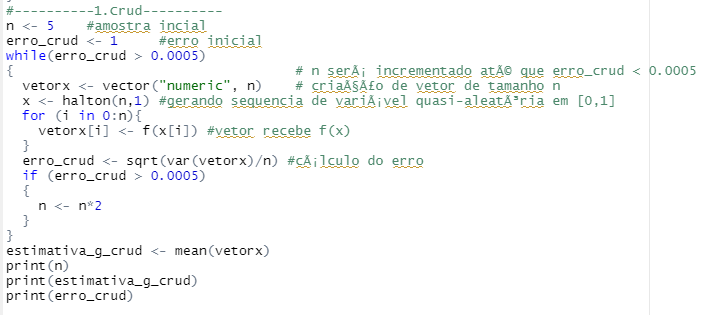
\includegraphics[scale=.5]{./Figuras/R_crud}\\
\end{center}
Dessa forma, obtivemos os seguintes resutados:\\
 $\hat{g} = 0.8066269; n = 81920;    \epsilon = 0.0003640106$

\section{Método Hit or Miss}

Neste método, geramos pares de pontos $(x_i,y_i)$ e escolhemos uma função auxiliar $h(x,y)$ de distribuição Bernoulli tal que 
\[
  h(x,y)= \left\{
    \begin{tabular}[]{cc}
     1 & \text{ se } $f(x) \geq y$,\\
     0 & \text{ se } $f(x) < y$.
    \end{tabular}
    \right.
  \]
  
  
  Assim, vamos estimar $g=\int_{0}^{1}\int_{0}^{1}h(x,y)dxdy$ como $\hat{g}=\frac{1}{n}\sum_{1}^{n}h(x_i,y_i)=\frac{n*}{n}$ e a estimativa da variância será dada por $s^2 = \dfrac{\hat{g}(1-\hat{g})}{n}$.
  
  
  Executamos o código abaixo no R e obtivemos os seguintes resultados:\\
\begin{center}
  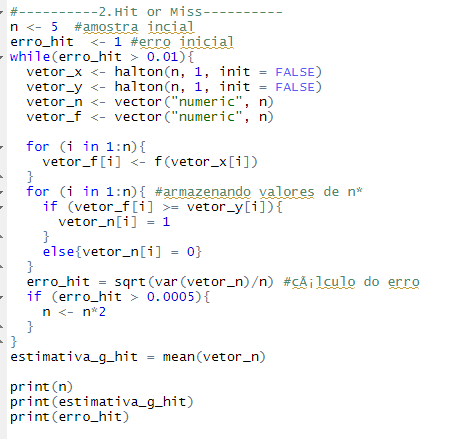
\includegraphics[scale=.45]{./Figuras/R_hit}\\
\end{center}  

 $\hat{g} = 0.6972237; n = 1310720;    \epsilon = 0.0004013213$

\section{Método Importance Sampling}



Neste método, escolhemos uma função auxiliar $k(x)$ que seja função de distribuição de probabilidade conhecida e se aproxime da $f(x)$.

$$
g = \int f(x)dx = \int\frac{f(x)}{k(x)} k(x)dx = \int \frac{f(x)}{k(x)}dK(x)
$$
$$
\hat{g} = \frac{1}{n}\sum_{1}^{n}\frac{f(x_i)}{k(x_i)}, x_i \sim k, i =1:n,s^2 = \frac{1}{n}\int\left(\frac{f(x)}{k(x)} - \hat{g}\right)^2dK(x)
$$


Vamos escolher a função de distribuição Beta($\alpha,\beta$), integrável, razoavelmente proporcional a $f(x)$ e cuja razão $f/Beta$ seja limitada no intervalo $[0,1]$, com $\alpha = 0.9$ e $\beta=1.1$ , ilustrada no gráfico abaixo, e armazenar os resultados de $f(x_i)/k(x_i)$ em um vetor e calcular sua média para chegar na aproximação $\hat{g}$.
\begin{center}
  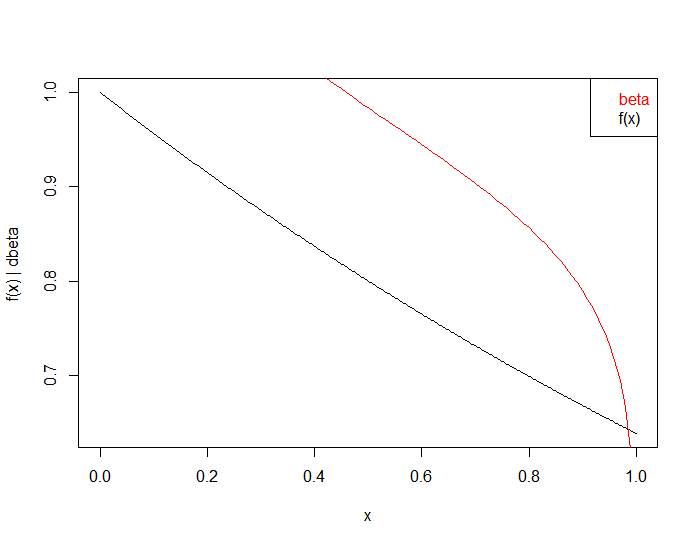
\includegraphics[scale=.55]{./Figuras/plot_beta}\\
\end{center}  
\begin{center}
  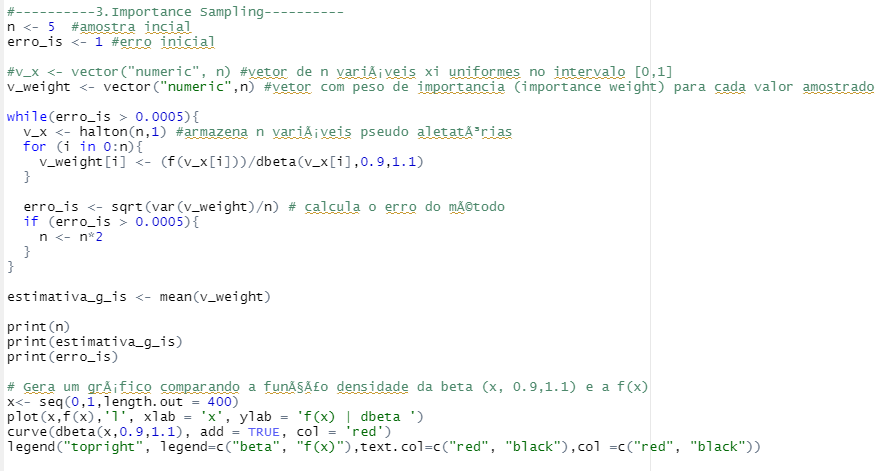
\includegraphics[scale=.5]{./Figuras/R_importance}\\
\end{center} 

Executando os comandos acima no R, obtivemos os seguintes resultados:\\
$\hat{g} = 0.7881357; n = 10240;    \epsilon = 0.0004244787$

\section{Método Control Variate}


No método Control Variate, escolhemos uma função $\varphi(x)$ de comportamento parecido com a $f(x)$, porém mais fácil de integrar.
$$
g = \int \varphi(x)dx + \int( f(x) - \varphi(x))dx  = g' + \int( f(x) - \varphi(x))dx
$$
Com os estimadores $\hat{g} = \frac{1}{n}\sum_{1}^{n}f(x_i)$ e $\hat{g'} = \frac{1}{n}\sum_{1}^{n}f(x_i)$ e a variância dada por $Var(\hat{g} - \hat{g'}) = Var(\hat{g})+Var(\hat{g'})-2Cov(\hat{g}, \hat{g'})$, o método é útil se as funções $f(x)$ e $\varphi(x)$ possuem forte correlação positiva.


Assim sendo, escolhemos a $\varphi(x) = 1 - 0.5x$, conforme imagem a seguir:
\begin{center}
  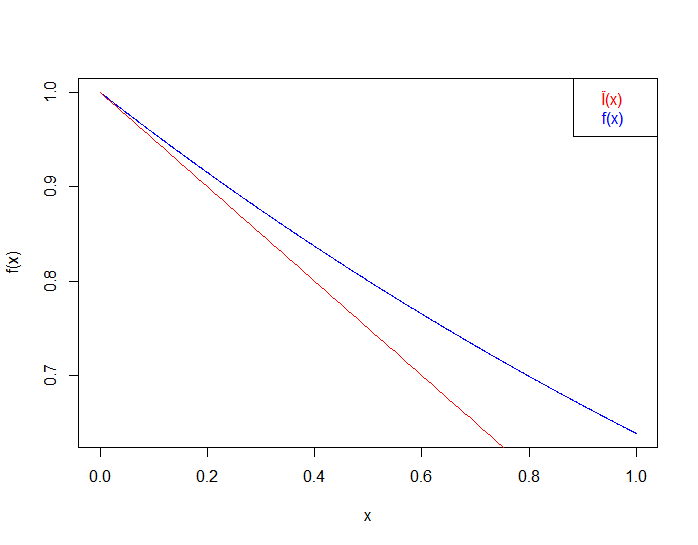
\includegraphics[scale=.4]{./Figuras/plot_phi}\\
\end{center}  


No R, armazenamos os valores de $f(x)$ e $\varphi(x)$ e suas diferenças em vetores. Assim, estimamos a integral de $f(x)$ como sendo a média de $\varphi(x)$  mais a média da diferença de $f(x)$ e $\varphi(x)$, conforme abaixo:
\begin{center}
  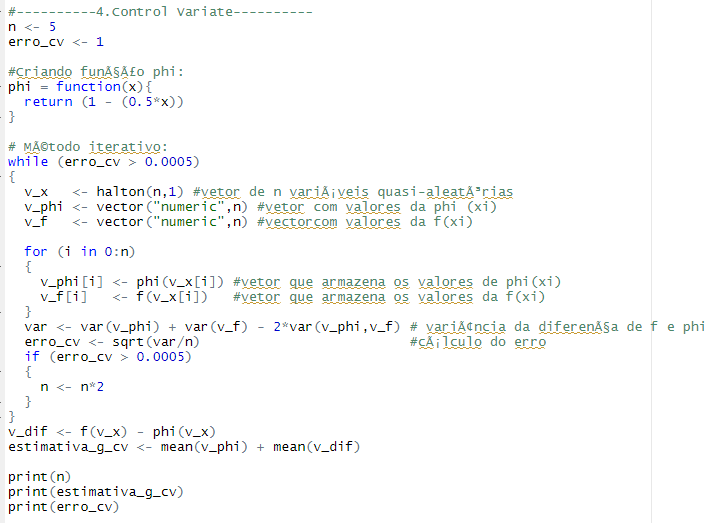
\includegraphics[scale=.35]{./Figuras/R_control}\\
\end{center} 
Executando os comandos acima no R, obtivemos os seguintes resultados:\\
$\hat{g} = 0.7855624; n = 1280;    \epsilon = 0.0004053953$

\section{Conclusões}

A implementação deste exercício foi muito parecida com o EP anterior, a diferença consistiu na ultilização do gerador quasi-aleatório \textit{halton} e, como era esperada uma convergência mais rápida, iniciamos com um n menor (n=5) para erro padrão $\leq$0.005.


Diferentemente do esperado na teoria, os métodos \textit{Crud} e \textit{Hit or Miss} demoraram mais para convergir em relação ao gerador pseudo-aleatório, porém apresentou pequena melhora na precisão da estimativa, que é proporcional a $\frac{1}{\sqrt{n}}$.


Os métodos \textit{Importance Sampling} e \textit{Control Variate} tiveram melhora na velocidade de convergência, piorando um pouco na precisão da estimativa, pois o erro padrão é inversamente proporcional a $\sqrt{n}$.

Destacamos abaixo uma comparação dos desempenhos dos métodos:

\begin{center}
\begin{tabular}{ |c|c|c|c| } 
 \hline
 Método                       & Estimativa & $n$  & Erro \\ 
 \hline
 \textit{Crud pseudo}                & 0.8064915  & 64000  & 0.0004124224 \\ 
 \textit{Crud quasi}                 & 0.8066269  & 81920  & 0.0003640106 \\ 
 \hline
 \textit{Hit or Miss pseudo}         & 0.8062969  & 1024000 & 0.0003905405 \\
 \textit{Hit or Miss quasi}          & 0.6972237  & 1310720 & 0.0004013213 \\
 \hline
 \textit{Importance Sampling pseudo} & 0.8160307  & 16000  & 0.0004419491 \\
 \textit{Importance Sampling quasi}  & 0.7881357  & 10240    &  0.0004244787\\
 \hline
 \textit{Control Variate pseudo}     & 0.8160307  & 8000  & 0.0004566607 \\
  \textit{Control Variate quasi}     & 0.7855624  & 1280 & 0.0004053953 \\
 \hline
\end{tabular}
\end{center}

%\bibliographystyle{plain}
%\bibliography{references}
\end{document}
